\documentclass[10pt,border=4pt]{standalone}
\usepackage{mathptmx}
\usepackage{amsmath,amssymb,bm}
\usepackage{tikz}
\usetikzlibrary{patterns,decorations.pathmorphing,decorations.pathreplacing,arrows.meta,fit,backgrounds,calc,positioning,shapes.geometric}
\definecolor{acc}{HTML}{0B5394}
\definecolor{accl}{HTML}{EAF0F7}
\definecolor{grp}{HTML}{F5F5F5}
\definecolor{org}{HTML}{C55A11}
\definecolor{orgl}{HTML}{FBEFE6}
\tikzset{
 dat/.style={draw=black,line width=0.6pt,fill=white,align=center,font=\small,inner sep=3pt,minimum height=0.85cm},
 lay/.style={draw=acc,line width=0.8pt,fill=accl,rounded corners=2pt,align=center,font=\small,inner sep=3pt,minimum height=0.85cm},
 cnd/.style={draw=org,line width=0.8pt,fill=orgl,rounded corners=2pt,align=center,font=\small,inner sep=3pt,minimum height=0.75cm},
 op/.style={circle,draw=black,line width=0.6pt,fill=white,inner sep=0.5pt,font=\small,minimum size=5mm},
 grpb/.style={draw=black!45,dashed,line width=0.6pt,rounded corners=3pt,inner sep=6pt},
 arr/.style={-{Latex[length=2.2mm,width=1.7mm]},line width=0.7pt},
 carr/.style={-{Latex[length=2.2mm,width=1.7mm]},line width=0.7pt,draw=org},
 shp/.style={font=\scriptsize,text=black!70,inner sep=1pt},
 lab/.style={font=\footnotesize,inner sep=1pt},
 ttl/.style={font=\small\bfseries,inner sep=0pt,anchor=west}
}
\newcommand{\xh}{\mathbf{x}_h}\newcommand{\xf}{\mathbf{x}_f}

\begin{document}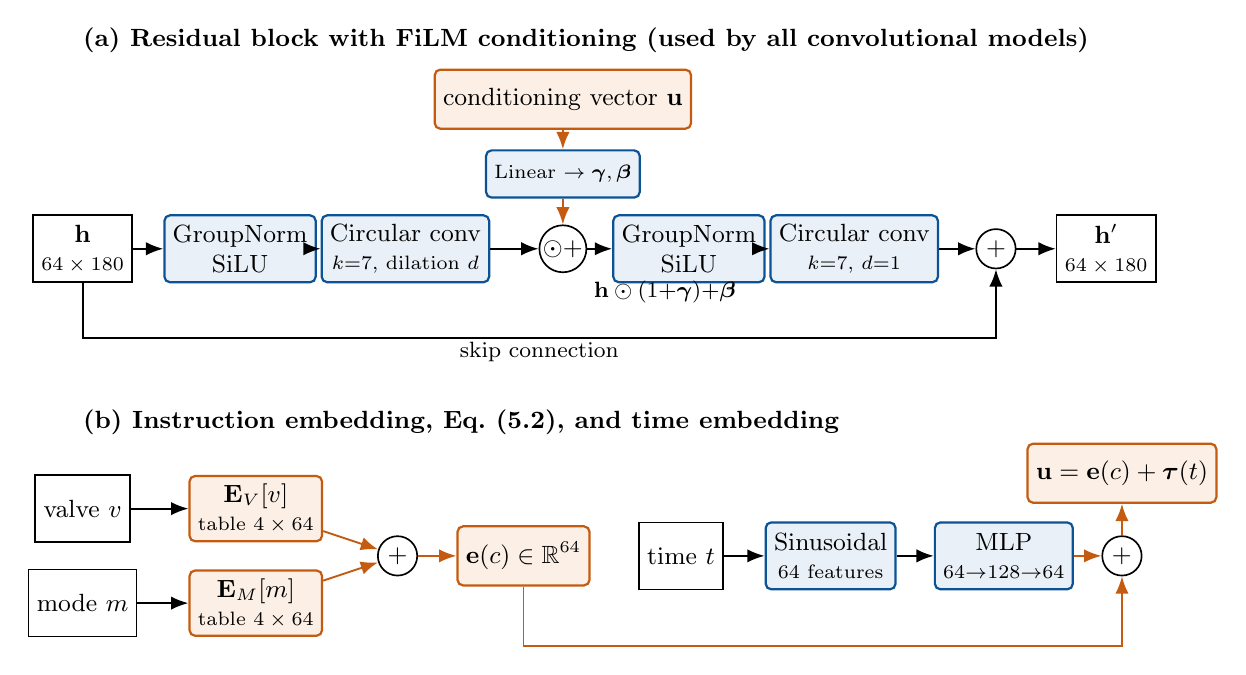
\begin{tikzpicture}[x=1cm,y=1cm]
% (a) residual block
\node[ttl] at (0,2.65) {(a) Residual block with FiLM conditioning (used by all convolutional models)};
\node[dat] (in) at (0,0) {$\mathbf{h}$\\[-1pt]\scriptsize $64\times180$};
\node[lay] (g1) at (2.0,0) {GroupNorm\\SiLU};
\node[lay] (c1) at (4.1,0) {Circular conv\\[-1pt]\scriptsize $k{=}7$, dilation $d$};
\node[op] (fm) at (6.1,0) {$\odot{+}$};
\node[lay] (g2) at (7.7,0) {GroupNorm\\SiLU};
\node[lay] (c2) at (9.8,0) {Circular conv\\[-1pt]\scriptsize $k{=}7$, $d{=}1$};
\node[op] (ad) at (11.6,0) {$+$};
\node[dat] (out) at (13.0,0) {$\mathbf{h}'$\\[-1pt]\scriptsize $64\times180$};
\draw[arr] (in)--(g1); \draw[arr] (g1)--(c1); \draw[arr] (c1)--(fm); \draw[arr] (fm)--(g2); \draw[arr] (g2)--(c2); \draw[arr] (c2)--(ad); \draw[arr] (ad)--(out);
\draw[arr] (in.south) -- ++(0,-0.7) -| node[lab,below,pos=0.25]{skip connection} (ad.south);
\node[cnd] (cv) at (6.1,1.9) {conditioning vector $\mathbf{u}$};
\node[lay,minimum height=0.6cm] (lin) at (6.1,0.95) {\scriptsize Linear $\rightarrow\boldsymbol\gamma,\boldsymbol\beta$};
\draw[carr] (cv)--(lin); \draw[carr] (lin)--(fm);
\node[lab,anchor=west] at (6.45,-0.55) {$\mathbf{h}\odot(1{+}\boldsymbol\gamma){+}\boldsymbol\beta$};
% (b) instruction and time embeddings
\node[ttl] at (0,-2.2) {(b) Instruction embedding, Eq.~(5.2), and time embedding};
\node[dat] (v) at (0,-3.3) {valve $v$};
\node[dat] (m) at (0,-4.5) {mode $m$};
\node[cnd] (ev) at (2.2,-3.3) {$\mathbf{E}_V[v]$\\[-1pt]\scriptsize table $4\times64$};
\node[cnd] (em) at (2.2,-4.5) {$\mathbf{E}_M[m]$\\[-1pt]\scriptsize table $4\times64$};
\node[op] (sum) at (4.0,-3.9) {$+$};
\node[cnd] (ec) at (5.6,-3.9) {$\mathbf{e}(c)\in\mathbb{R}^{64}$};
\draw[arr] (v)--(ev); \draw[arr] (m)--(em); \draw[carr] (ev)--(sum); \draw[carr] (em)--(sum); \draw[carr] (sum)--(ec);
\node[dat] (t) at (7.6,-3.9) {time $t$};
\node[lay] (sin) at (9.5,-3.9) {Sinusoidal\\[-1pt]\scriptsize 64 features};
\node[lay] (mlp) at (11.7,-3.9) {MLP\\[-1pt]\scriptsize $64{\to}128{\to}64$};
\node[op] (s2) at (13.2,-3.9) {$+$};
\draw[arr] (t)--(sin); \draw[arr] (sin)--(mlp); \draw[carr] (mlp)--(s2);
\draw[carr] (ec.south) -- ++(0,-0.75) -| (s2.south);
\node[cnd] (u) at (13.2,-2.85) {$\mathbf{u}=\mathbf{e}(c)+\boldsymbol\tau(t)$};
\draw[carr] (s2)--(u);
\end{tikzpicture}\end{document}
